\documentclass[12pt, a4paper]{article}

\usepackage{amsmath}
\usepackage{amsfonts}
\usepackage{amssymb}
\usepackage{graphicx}
\usepackage{float}
\usepackage{listings}
\usepackage{rotating}
\usepackage{tikz}
\usepackage{verbatim}
\pdfgentounicode=1
\pdfmapline{+cyberb@Unicode@  <cyberbit.ttf}

\begin{document}

\title{PBMath}
\author{P. Baillehache}
\date{\today}
\maketitle

\tableofcontents

\section*{Introduction}

PBMath is C library providing mathematical structures and functions.\\ 

The \begin{ttfamily}VecFloat\end{ttfamily} structure and its functions can be used to manipulate vectors of float values.\\

The \begin{ttfamily}Gauss\end{ttfamily} structure and its functions can be used to get values of the Gauss function and random values distributed accordingly with a Gauss distribution.\\

The \begin{ttfamily}Smoother\end{ttfamily} functions can be used to get values of the SmoothStep and SmootherStep functions.\\

\section{Interface}

\begin{scriptsize}
\begin{ttfamily}
\verbatiminput{../pbmath.h}
\end{ttfamily}
\end{scriptsize}

\section{Code}

\begin{scriptsize}
\begin{ttfamily}
\verbatiminput{../pbmath.c}
\end{ttfamily}
\end{scriptsize}

\section{Makefile}

\begin{scriptsize}
\begin{ttfamily}
\verbatiminput{../Makefile}
\end{ttfamily}
\end{scriptsize}

\section{Usage}

\begin{scriptsize}
\begin{ttfamily}
\verbatiminput{../main.c}
\end{ttfamily}
\end{scriptsize}

Output:\\
\begin{scriptsize}
\begin{ttfamily}
\verbatiminput{../output.txt}
\end{ttfamily}
\end{scriptsize}

vecshort.txt:\\
\begin{scriptsize}
\begin{ttfamily}
\verbatiminput{../vecshort.txt}
\end{ttfamily}
\end{scriptsize}

vecfloat.txt:\\
\begin{scriptsize}
\begin{ttfamily}
\verbatiminput{../vecfloat.txt}
\end{ttfamily}
\end{scriptsize}

smoother functions:\\
\begin{center}
\begin{figure}[H]
\centering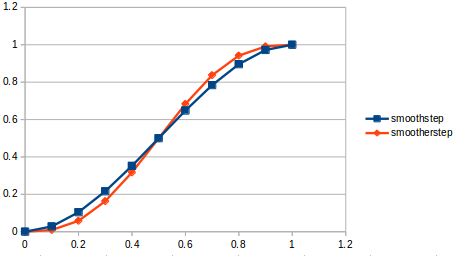
\includegraphics[width=6cm]{./smoother.png}\\
\end{figure}
\end{center}

gauss function (mean:0.0, sigma:1.0):\\
\begin{center}
\begin{figure}[H]
\centering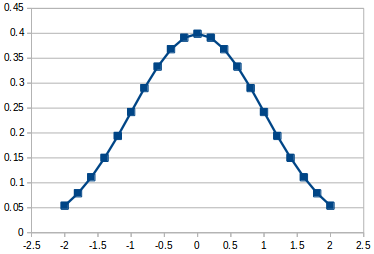
\includegraphics[width=6cm]{./gauss.png}\\
\end{figure}
\end{center}

gauss rand function (mean:1.0, sigma:0.5):\\
\begin{center}
\begin{figure}[H]
\centering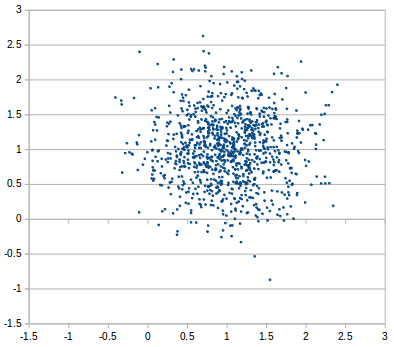
\includegraphics[width=6cm]{./gaussrnd.png}\\
\end{figure}
\end{center}

\end{document}


